% Chapter Template

\chapter{Hierarchical clustering of data}
% Main chapter title

\label{Chapter3} % Change X to a consecutive number; for referencing this chapter elsewhere, use \ref{ChapterX}

\lhead{Chapter 3. \emph{Hierarchical clustering of data}} 

\section{Introduction}

In this chapter, I cluster vastly different types of data using the
normalized compression distance. I introduce a lightweight alternative to
the CompLearn Toolkit \ref{CompLearn}. My clustering tool uses common
Python and R libraries, and is less than a hundred lines of code.

To explain the method, I first cluster mitochondrial gene sequences of
mammals.

\section{Evolution of placental mammals}

Reconstructing an evolutionary tree has intuitive appeal. It should lend
itself well to hierarchical clustering, since species emerge from common
ancestors. And, within biology, there is agreement on what the true
phylogeny tree is: the brown bear and polar bear are closely related, etc.
Only higher up on the tree there is ongoing debate. Do the primates first
join with the rodents, or are they more closely connected to the
ferungulates? 

All materials were taken from the GenBank database \cite{GenBank}.

In \cite{Cao1998}, the authors estimate the likelihood of phylogeny trees
based on 12 mitochondrial proteins of 20 placental mammals: rat
(\emph{Rattus norvegicus}), house mouse (\emph{Mus musculus}), grey seal
(\emph{Halichoerus grypus}), harbor seal (\emph{Phoca vitulina}), cat
(\emph{Felis catus}), white rhino (\emph{Ceratotherium simum}), horse
(\emph{Equus caballus}), finback whale (\emph{Balaenoptera physalus}),
blue whale (\emph{Balaenoptera musculus}), cow (\emph{Bos taurus}), gibbon
(\emph{Hylobates lar}), gorilla (\emph{Gorilla gorilla}), human
(\emph{Homo sapiens}), chimpanzee (\emph{Pan troglodytes}), pygmy
chimpanzee (\emph{Pan paniscus}), orangutan (\emph{Pongo pygmaeus}),
Sumatran orangutan (\emph{Pongo abelii}), using opossum (\emph{Didelphis
virginiana}), wallaroo (\emph{Macropus robustus}), and the platypus
(\emph{Ornithorhynchus anatinus}).

In \cite{Cilibrasi2005}, 4 more mammals were added: Australian echidna
(\emph{Tachyglossus aculeatus}), brown bear (\emph{Ursus arctos}), polar
bear (\emph{Ursus maritimus}), and the common carp (\emph{Cyprinus
carpio}). The common carp is not a mammal and is used as an outgroup. It
should join the phylogeny tree at the very top.

The authors of \cite{Cilibrasi2005} cluster the complete mitochondrial
genome sequences with the normalized compression distance. They use
a clustering algorithm described by them in
\cite{Cilibrasi2011}. The algorithm tries to optimize a global criterion,
namely the (normalized) summed weights of all consistent quartet
topologies (layouts of groups of four items). In a binary tree, only one
of three possible pairings of four items ($ab|cd$, $ac|bd$, $ad|bc$) is
\emph{consistent}, in the sense that you can connect the two pairs without
crossing paths. The sum of the distances (in this case, $\text{NCD}$s)
between the items in the consistent pairs is the contribution of quartet
$abcd$ to the tree score.

This method works especially well if the items you're trying to cluster
result from an evolutionary process, since then (without corruption of
data) there should exist an evolutionary tree that embeds all the most
likely quartet topologies, and, given enough time, the heuristic presented
in \cite{Cilibrasi2011} finds the true tree.

Now, we will cluster the same 24 genome sequences with a much simpler
algorithm (average linkage) and compare results.

\subsection{Distance matrix}

The distance matrix contains the distances between all pairs of items.
Entry $i$, $j$ is the distance between item $i$ and item $j$, i.e.
$\text{NCD}(i, j)$. The distance matrix for the 24 animals is displayed in
table \ref{table:distance_matrix}.

\begin{table}[ht]
\scalebox{0.50}{
\begin{tabular}{rrrrrrrrrrrrrrrrrrrrrrrrr}
  \hline
blueWhale & 0.01 & 0.72 & 0.86 & 0.67 & 0.78 & 0.60 & 0.83 & 0.24 & 0.81 & 0.80 & 0.67 & 0.66 & 0.62 & 0.78 & 0.77 & 0.82 & 0.81 & 0.77 & 0.83 & 0.70 & 0.79 & 0.78 & 0.83 & 0.63 \\ 
  brownBear & 0.71 & 0.01 & 0.89 & 0.63 & 0.84 & 0.72 & 0.85 & 0.69 & 0.84 & 0.82 & 0.56 & 0.56 & 0.69 & 0.81 & 0.80 & 0.84 & 0.84 & 0.82 & 0.84 & 0.11 & 0.82 & 0.83 & 0.84 & 0.64 \\ 
  carp & 0.87 & 0.88 & 0.01 & 0.88 & 0.89 & 0.87 & 0.89 & 0.89 & 0.89 & 0.89 & 0.89 & 0.88 & 0.87 & 0.88 & 0.86 & 0.88 & 0.89 & 0.89 & 0.90 & 0.88 & 0.88 & 0.89 & 0.88 & 0.88 \\ 
  cat & 0.67 & 0.59 & 0.87 & 0.01 & 0.79 & 0.68 & 0.84 & 0.69 & 0.79 & 0.79 & 0.59 & 0.57 & 0.61 & 0.81 & 0.77 & 0.80 & 0.80 & 0.80 & 0.82 & 0.60 & 0.75 & 0.81 & 0.78 & 0.59 \\ 
  chimpanzee & 0.78 & 0.83 & 0.90 & 0.81 & 0.01 & 0.77 & 0.87 & 0.82 & 0.49 & 0.34 & 0.80 & 0.79 & 0.79 & 0.29 & 0.84 & 0.88 & 0.47 & 0.17 & 0.89 & 0.83 & 0.84 & 0.47 & 0.86 & 0.80 \\ 
  cow & 0.61 & 0.73 & 0.87 & 0.68 & 0.78 & 0.01 & 0.84 & 0.61 & 0.79 & 0.78 & 0.66 & 0.66 & 0.62 & 0.81 & 0.77 & 0.82 & 0.81 & 0.77 & 0.84 & 0.71 & 0.76 & 0.81 & 0.81 & 0.62 \\ 
  echidna & 0.84 & 0.87 & 0.89 & 0.85 & 0.85 & 0.83 & 0.01 & 0.86 & 0.85 & 0.86 & 0.87 & 0.87 & 0.84 & 0.88 & 0.81 & 0.81 & 0.87 & 0.85 & 0.55 & 0.87 & 0.84 & 0.86 & 0.84 & 0.83 \\ 
  finWhale & 0.25 & 0.72 & 0.89 & 0.71 & 0.81 & 0.62 & 0.85 & 0.01 & 0.81 & 0.82 & 0.70 & 0.69 & 0.64 & 0.81 & 0.80 & 0.84 & 0.80 & 0.78 & 0.85 & 0.72 & 0.81 & 0.81 & 0.85 & 0.64 \\ 
  gibbon & 0.83 & 0.85 & 0.90 & 0.81 & 0.51 & 0.81 & 0.88 & 0.85 & 0.01 & 0.51 & 0.82 & 0.83 & 0.81 & 0.50 & 0.85 & 0.89 & 0.53 & 0.50 & 0.90 & 0.85 & 0.85 & 0.54 & 0.87 & 0.79 \\ 
  gorilla & 0.79 & 0.81 & 0.90 & 0.82 & 0.35 & 0.79 & 0.88 & 0.83 & 0.50 & 0.01 & 0.79 & 0.82 & 0.83 & 0.35 & 0.83 & 0.89 & 0.46 & 0.35 & 0.87 & 0.82 & 0.82 & 0.47 & 0.88 & 0.80 \\ 
  graySeal & 0.69 & 0.56 & 0.88 & 0.60 & 0.79 & 0.66 & 0.84 & 0.69 & 0.79 & 0.80 & 0.01 & 0.16 & 0.64 & 0.80 & 0.77 & 0.82 & 0.80 & 0.78 & 0.85 & 0.55 & 0.78 & 0.80 & 0.80 & 0.61 \\ 
  harborSeal & 0.67 & 0.54 & 0.88 & 0.58 & 0.78 & 0.64 & 0.85 & 0.69 & 0.80 & 0.80 & 0.16 & 0.01 & 0.61 & 0.79 & 0.76 & 0.83 & 0.77 & 0.77 & 0.84 & 0.54 & 0.77 & 0.77 & 0.80 & 0.60 \\ 
  horse & 0.63 & 0.65 & 0.88 & 0.63 & 0.76 & 0.62 & 0.85 & 0.64 & 0.77 & 0.79 & 0.62 & 0.60 & 0.01 & 0.79 & 0.78 & 0.81 & 0.78 & 0.78 & 0.83 & 0.66 & 0.76 & 0.79 & 0.80 & 0.49 \\ 
  human & 0.78 & 0.83 & 0.88 & 0.83 & 0.30 & 0.79 & 0.87 & 0.80 & 0.50 & 0.35 & 0.82 & 0.82 & 0.78 & 0.01 & 0.82 & 0.87 & 0.46 & 0.30 & 0.88 & 0.83 & 0.82 & 0.46 & 0.86 & 0.78 \\ 
  mouse & 0.77 & 0.79 & 0.86 & 0.76 & 0.81 & 0.76 & 0.81 & 0.80 & 0.81 & 0.82 & 0.77 & 0.76 & 0.75 & 0.83 & 0.01 & 0.78 & 0.83 & 0.82 & 0.83 & 0.78 & 0.54 & 0.83 & 0.77 & 0.74 \\ 
  opossum & 0.82 & 0.81 & 0.87 & 0.80 & 0.87 & 0.81 & 0.84 & 0.82 & 0.87 & 0.88 & 0.82 & 0.82 & 0.81 & 0.87 & 0.80 & 0.01 & 0.88 & 0.87 & 0.84 & 0.82 & 0.82 & 0.88 & 0.68 & 0.83 \\ 
  orangutan & 0.80 & 0.83 & 0.90 & 0.82 & 0.46 & 0.82 & 0.88 & 0.80 & 0.52 & 0.46 & 0.82 & 0.79 & 0.83 & 0.45 & 0.84 & 0.88 & 0.01 & 0.47 & 0.89 & 0.83 & 0.83 & 0.25 & 0.86 & 0.82 \\ 
  pigmyChimpanzee & 0.77 & 0.81 & 0.90 & 0.81 & 0.17 & 0.77 & 0.88 & 0.81 & 0.49 & 0.34 & 0.82 & 0.79 & 0.79 & 0.29 & 0.83 & 0.87 & 0.47 & 0.01 & 0.89 & 0.81 & 0.83 & 0.47 & 0.86 & 0.78 \\ 
  platypus & 0.83 & 0.85 & 0.89 & 0.86 & 0.89 & 0.82 & 0.56 & 0.84 & 0.89 & 0.87 & 0.84 & 0.84 & 0.87 & 0.87 & 0.83 & 0.82 & 0.88 & 0.88 & 0.01 & 0.85 & 0.84 & 0.89 & 0.84 & 0.85 \\ 
  polarBear & 0.70 & 0.10 & 0.89 & 0.62 & 0.81 & 0.70 & 0.86 & 0.71 & 0.84 & 0.81 & 0.56 & 0.56 & 0.66 & 0.82 & 0.79 & 0.83 & 0.82 & 0.81 & 0.85 & 0.01 & 0.78 & 0.82 & 0.82 & 0.65 \\ 
  rat & 0.78 & 0.82 & 0.89 & 0.75 & 0.80 & 0.76 & 0.83 & 0.78 & 0.81 & 0.82 & 0.79 & 0.77 & 0.74 & 0.82 & 0.55 & 0.82 & 0.81 & 0.83 & 0.86 & 0.82 & 0.01 & 0.81 & 0.84 & 0.75 \\ 
  sumatranOrangutan & 0.78 & 0.82 & 0.89 & 0.80 & 0.47 & 0.80 & 0.86 & 0.79 & 0.52 & 0.47 & 0.80 & 0.80 & 0.77 & 0.44 & 0.84 & 0.87 & 0.24 & 0.47 & 0.88 & 0.82 & 0.82 & 0.01 & 0.87 & 0.78 \\ 
  wallaroo & 0.81 & 0.82 & 0.87 & 0.80 & 0.85 & 0.81 & 0.85 & 0.83 & 0.86 & 0.86 & 0.80 & 0.79 & 0.81 & 0.85 & 0.81 & 0.68 & 0.86 & 0.85 & 0.83 & 0.83 & 0.82 & 0.87 & 0.01 & 0.80 \\ 
  whiteRhinoceros & 0.64 & 0.66 & 0.89 & 0.65 & 0.78 & 0.64 & 0.86 & 0.65 & 0.78 & 0.79 & 0.61 & 0.61 & 0.51 & 0.79 & 0.78 & 0.84 & 0.82 & 0.79 & 0.86 & 0.68 & 0.77 & 0.81 & 0.82 & 0.01 \\ 
   \hline
\end{tabular} }
\caption{Distance matrix of genome sequences of 24 animals. To obtain the
$\text{NCD}$, I used ruby-xz, the Ruby binding to compressor liblzma, with settings
\texttt{compression\underline{{ }}level = 9}, \texttt{extreme = true},
\texttt{check = :none}. }
\label{table:distance_matrix} \end{table}

\subsection{Clustering method}

In hierarchical clustering, the goal is to build a hierarchy of clusters from a distance matrix. The hierarchy can be displayed as a binary tree. One of the simplest ways to do this is to put every object in its own cluster, and then merge greedily based on a linkage criterion, until all items have been merged into a single cluster.

In single linkage, at each step the two clusters are merged with the smallest pairwise distance. This is also called \emph{nearest neighbor} clustering.

In complete linkage, or \emph{farthest neighbor} clustering, at each step the two clusters with the largest pairwise distance are merged.

Average linkage is a compromise between single and complete linkage. The distance between two clusters is defined as the average between the pairwise distances, i.e.

$$ d(A, B) = \frac{1}{|A||B|} \sum_{a \in A}\sum_{b \in B} d(a, b) $$

\subsection{Phylogeny tree}

Figure \ref{figure:dendrogram_mammals} shows the phylogeny tree obtained by average link clustering.

\begin{figure}[h!]
  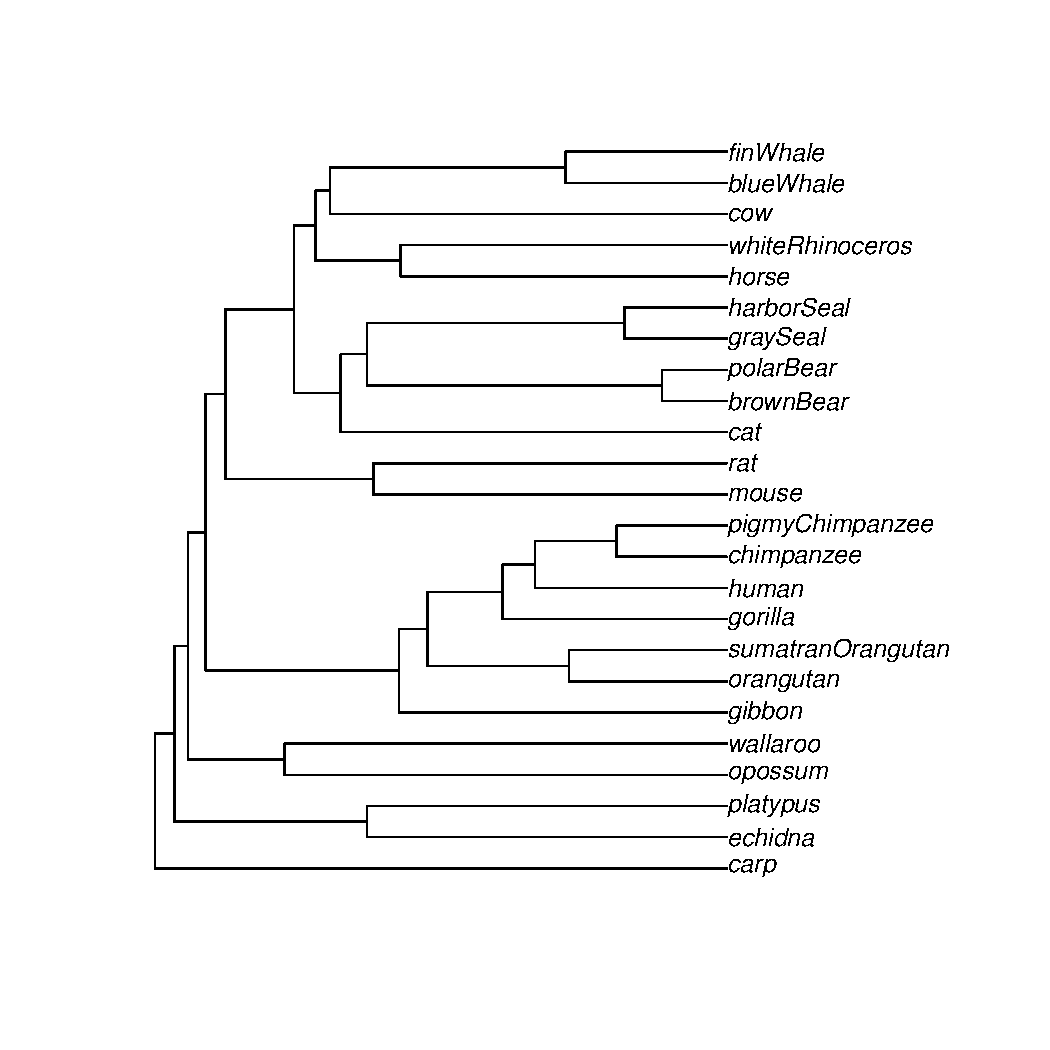
\includegraphics[scale=0.7]{24-mammals-average.pdf}
  \caption{Result of average linkage clustering of the distance matrix shown in table \ref{table:distance_matrix}. The height at which clusters join is proportional to the distance between them. }
  \label{figure:dendrogram_mammals}
\end{figure}

Comparison with \cite{Cao1998} shows that the dendrogram in this paper is a little bit off. Here, $((\text{finWhale}, \text{blueWhale}), \text{cow})$ joins $(\text{whiteRhinoceros}, \text{horse})$ first, while in the cited paper $((\text{harborSeal}, \text{greySeal}), \text{cat})$ first joins $(\text{horse}, \text{rhinoceros})$. Also, higher up in the tree, in this paper, the rodents join the ferungulates, and then the primates join, while in the cited paper the primates and ferungulates join first, and then the rodents join.

\cite{Cilibrasi2005}, which also uses NCD, but clusters with an algorithm described in \cite{Cilibrasi2011}, does not make these mistakes. But, the algorithm they use works especially well for evolutionary data, and they attain a global fitness score of $S(T) = 0.996$ for their tree $T$, which is exceptionally high. Other trees, containing, for example, random correlated data, have $S(T) = 0.905$ for the best found tree.

\section{Random correlated data}

In this section, we will cluster files containing random bytes, which we have partially correlated, so we know what the clustering should be like. This method of validation was taken from \cite{Cilibrasi2005}. All byte sequences have been generated with the random\_bytes function of the Ruby library SecureRandom.

Let \emph{tags} $a$, $b$, $c$ be blocks of 1000 random bytes. We create file $a$ in the following way: generate 80.000 random bytes, and at 10 distinct positions (picked from $0 \dots 79$) replace a 1000 byte block with tag $a$. To create file $ab$, we insert tag $a$ at 10 distinct positions, then insert tag $b$ at 10 distinct positions, possibly overwriting some of the earlier insertions of tag $a$. In this way, we create files $a$, $b$, $c$, $ab$, $ac$, $bc$, and $abc$. The clustering is shown in \ref{figure:7_artificial_files}.

I opted for single linkage clustering, i.e. the distance between clusters $A$ and $B$ is $d(A, B) = \min_{a \in A, b \in B} \text{d}(a, b)$, because it shows the fact that $ab$, $ac$ and $bc$ have about the same distance to $abc$, while $a$, $b$ and $c$ are farther away, but also at an even distance, exactly as you would expect.

\begin{figure}[h!]
  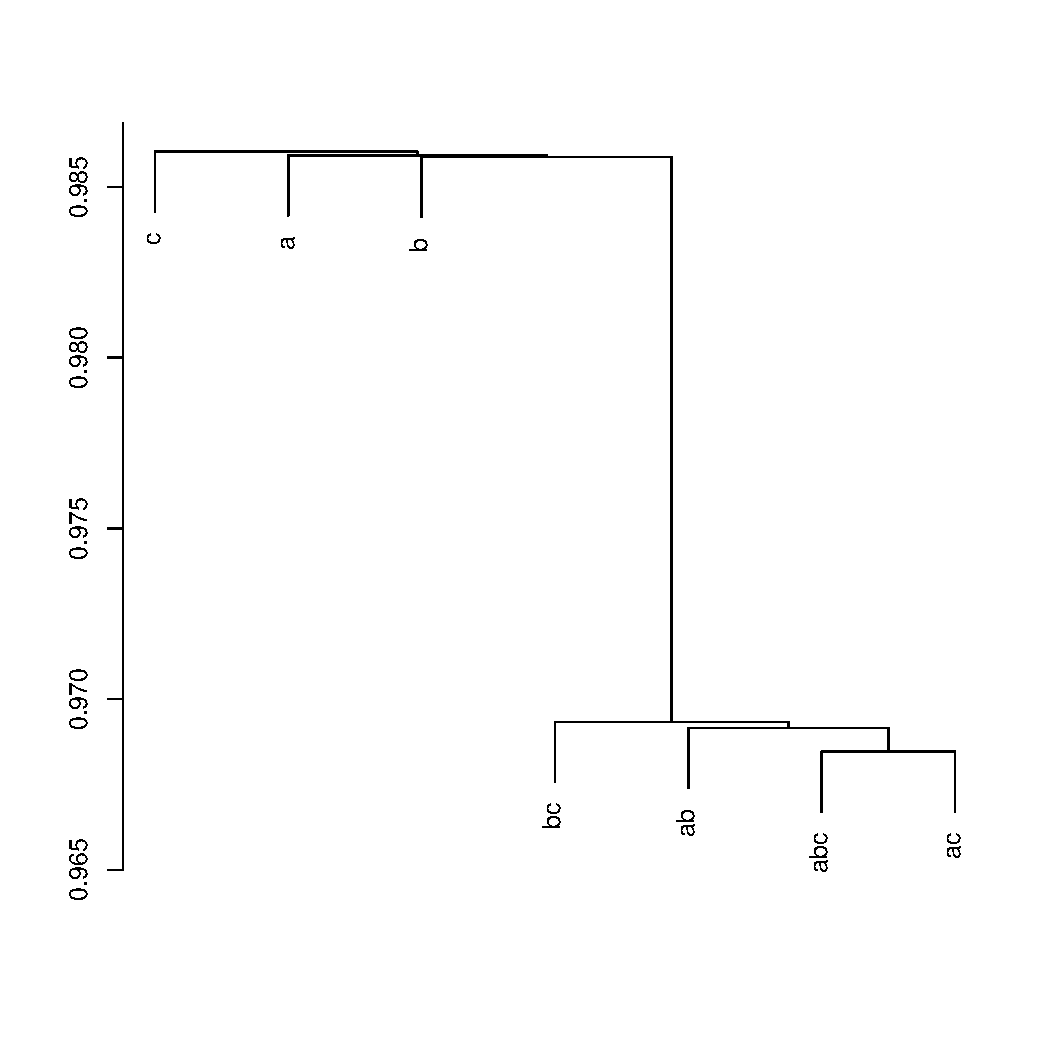
\includegraphics[scale=0.7]{7-artificial-files-single.pdf}
  \caption{Single link clustering of seven 80 kB files containing random bytes, which are partially correlated. The height at which clusters join is the distance between them, according to the linkage criterion.}
  \label{figure:7_artificial_files}
\end{figure}

In figure \ref{figure:22_artificial_files}, the experiment is repeated with 22 files, mimicking the experiment done in \cite{Cilibrasi2005}. The result is what you would expect, and you could argue that this clustering is more insightful than the quartet tree method, since it shows the degree in which two clusters are related. $abcd$ is closer to $abce$ than $jk$ is to any file labeled by more than two tags, for example.

\begin{figure}[h!]
  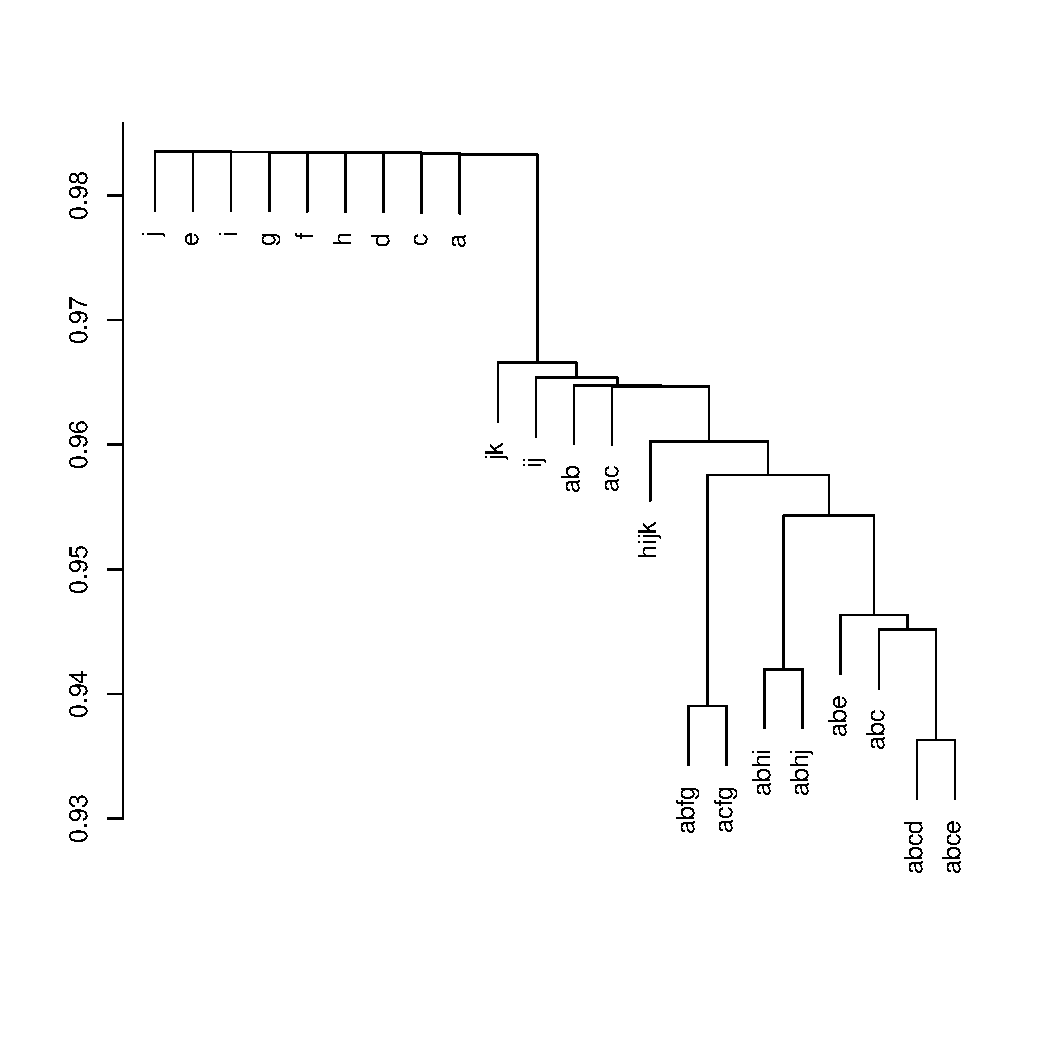
\includegraphics[scale=0.7]{22-artificial-files-single.pdf}
  \caption{Single link clustering of twenty-two 80 kB files containing random bytes, which are partially correlated.}
  \label{figure:22_artificial_files}
\end{figure}

\section{Literature}

We proceed to clustering of utf-8 files of books obtained from \url{www.gutenberg.org}. Here, the result is hard to validate, except for human intuition. The books used in this experiment are (1) A Week on the Concord and Merrimack Rivers, (2) Walden, and On The Duty of Civil Disobedience, both by Thoreau, (3) The Adventures of Sherlock Holmes, (4) The Hound of the Baskervilles, both by Doyle, (5) The Beautiful and the Damned, (6) This Side of Paradise, both by Fitzgerald, (7) Sons and Lovers, (8) White Peacock, both by Lawrence. The result is shown in figure \ref{figure:8_books}.

\begin{figure}[h!]
  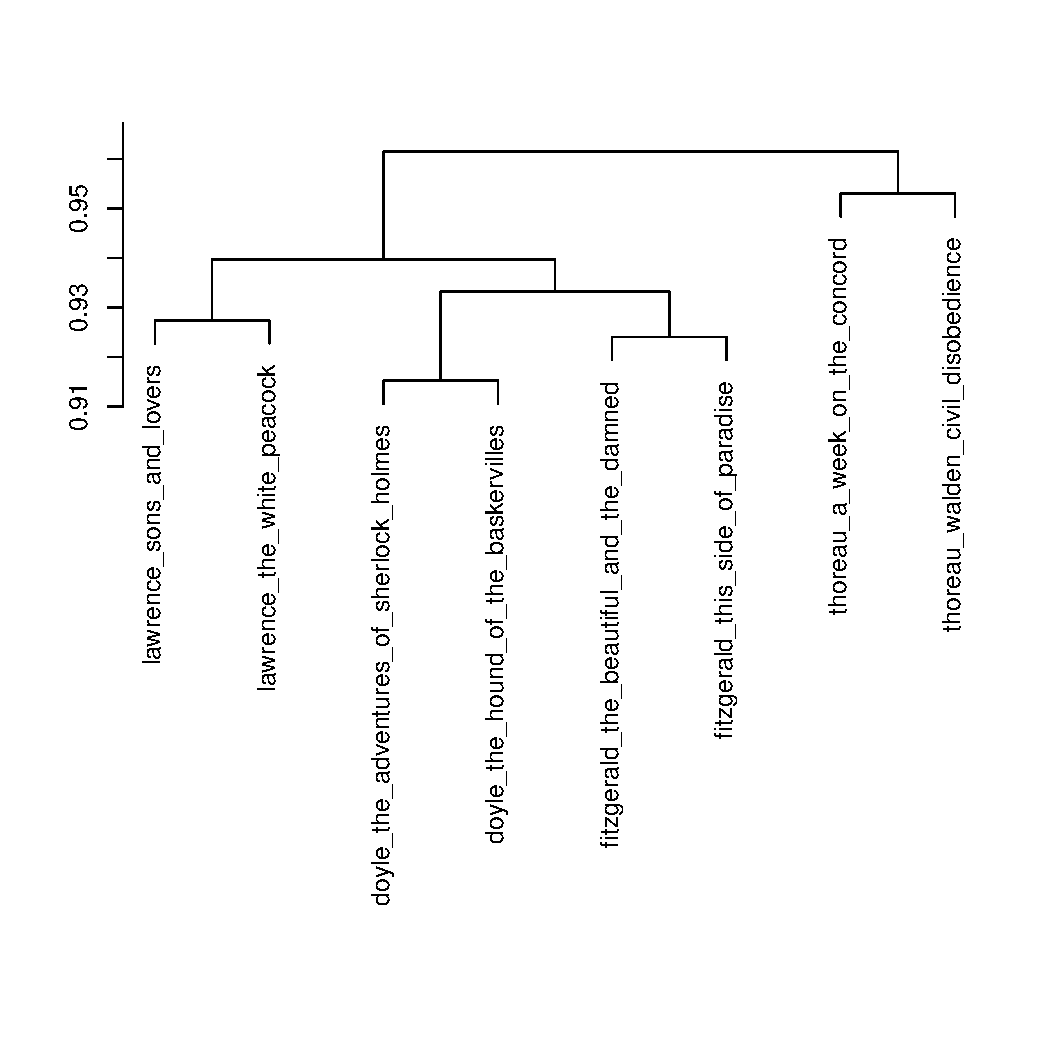
\includegraphics[scale=0.7]{literature-average.pdf}
  \caption{Average link clustering of eight books by english and american writers in utf-8 format.}
  \label{figure:8_books}
\end{figure}


\section{Source files}

We cluster ten files from the Ruby standard library \cite{ruby} at commit \texttt{c722f8ad1d}, ten files from the Clojure standard library \cite{clojure} at commit \texttt{41af6b24dd} and ten files from the Glasgow Haskell Compiler 6.10.1 \cite{ghc}. All comments and blank lines were stripped. This removes, among other things, copyright notices which were shared by files belonging to the same library. The result is shown in figure \ref{figure:30_source_files}. No preprocessing gives similar results.

\begin{figure}[h!]
  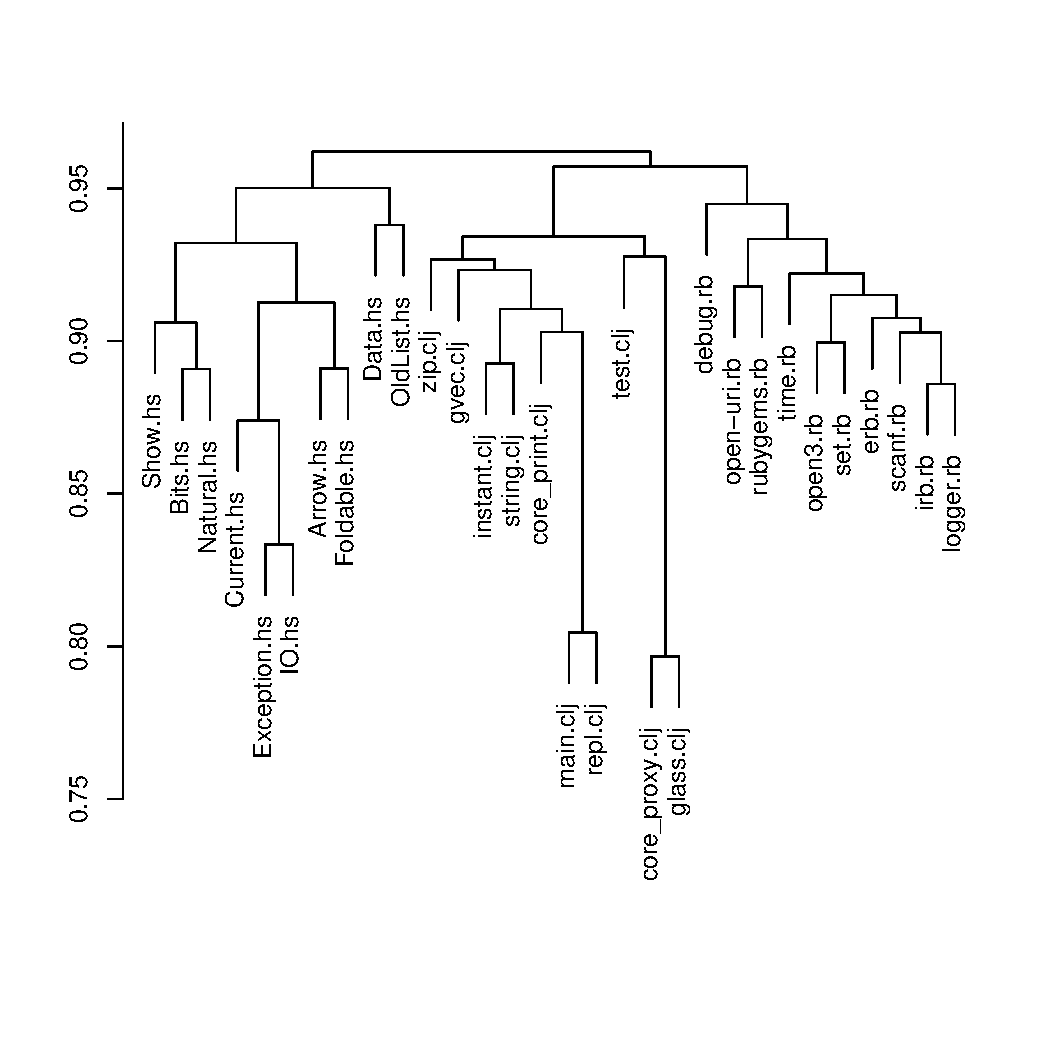
\includegraphics[scale=0.7]{30-source-files-no-comments-average.pdf}
  \caption{Average link clustering of 30 source files. The comments and blank lines were stripped using the \emph{cloc} utility.}
  \label{figure:30_source_files}
\end{figure}


